\subsection{time-series}
\label{sec:time-series}
\begin{quote}
  A time-series is a sequence of data
  points that occur in successive order over some period of time.
\end{quote}
\cite{Hayes}

In a time-series, time is often the independent variable.
Examples of time-series are weather data, stock markets, sound level samples.
The time $t$ usually ranges over a discrete index set and is often equally spaced.

\subsubsection{Properties}
A time-series has several properties:


\textbf{Stationarity}
A time-series is stationary if its statistical properties do not change over time.
In other words, if it has a variance, mean, and covariance independent of time.

\cite{RobJHyndman2014} defines stationarity more formally:
\begin{definition}
  $X_t$ is a stationary time-series
  $x_1, ..., x_n, if \forall_s \in \mathbb{R} :$
  the distribution of $(x_t, ..., x_{t+s})$ is equal
\end{definition}

\begin{figure}[h!]
  \centering
  \caption{Examples of stationarity}
  \label{fig:time-series-examples-stationary-and-non-stationary}
  \begin{subfigure}[b]{0.4\textwidth}
    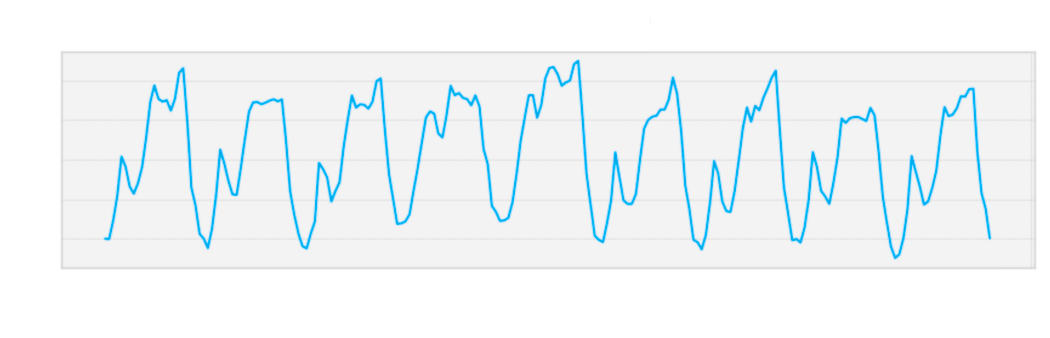
\includegraphics[width=\textwidth]{./figs/illustrations/time-series_example_stationary.png}
    \hfill
    \caption{A stationary Time-Series}
    \label{fig:stationary-time-series}
  \end{subfigure}
  \begin{subfigure}[b]{0.4\textwidth}
    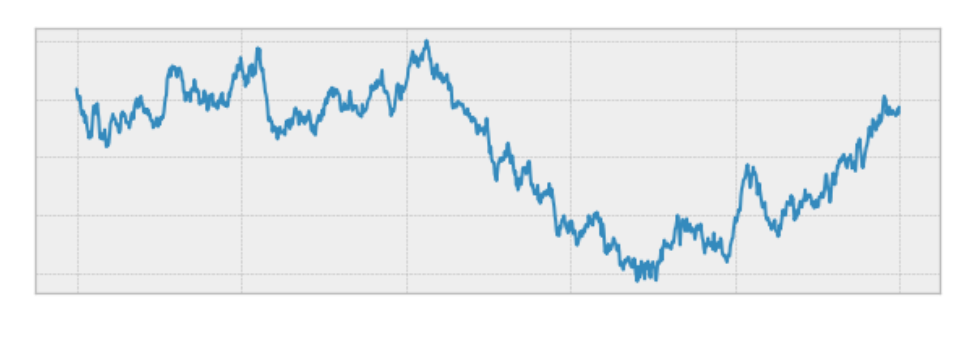
\includegraphics[width=\textwidth]{./figs/illustrations/time-series_example_non-stationary.png}
    \hfill
    \caption{Non-stationary Time-Series}
    \label{fig:non-stationary-time-series}
  \end{subfigure}
\end{figure}

\textbf{Seasonality}
If the time-series follows periodic fluctuations, like how electricity usage varies during 24 hours,
then it has seasonality. \Cref{fig:stationary-time-series} shows a clear cycle where
a clear pattern repeats over again.

\textbf{Autocorrelation}
If a time-series has a strong autocorrelation, then there is a big
correlation between observations with a time lag between them.

\textbf{Trends}
When a time-series has a deterministic component proportionate to the time period it has a trend.
In simpler terms, if a time-series plot seems to center around an increasing or decreasing line, it suggests the presence of a trend.
\Cref{fig:example-time-series-decomposed} show a series with a clear growing trend.

\textbf{time-series}
Cycles differ from seastime-seriesause the period does not have to be fixed.


\textbf{Level}
The level of a time-series is equal to the mean. If a time-series has a trend
then the level is changing.



\begin{figure}[h!]
  \centering
  \caption{A Time-Series decomposed}
  \label{fig:example-time-series-decomposed}
  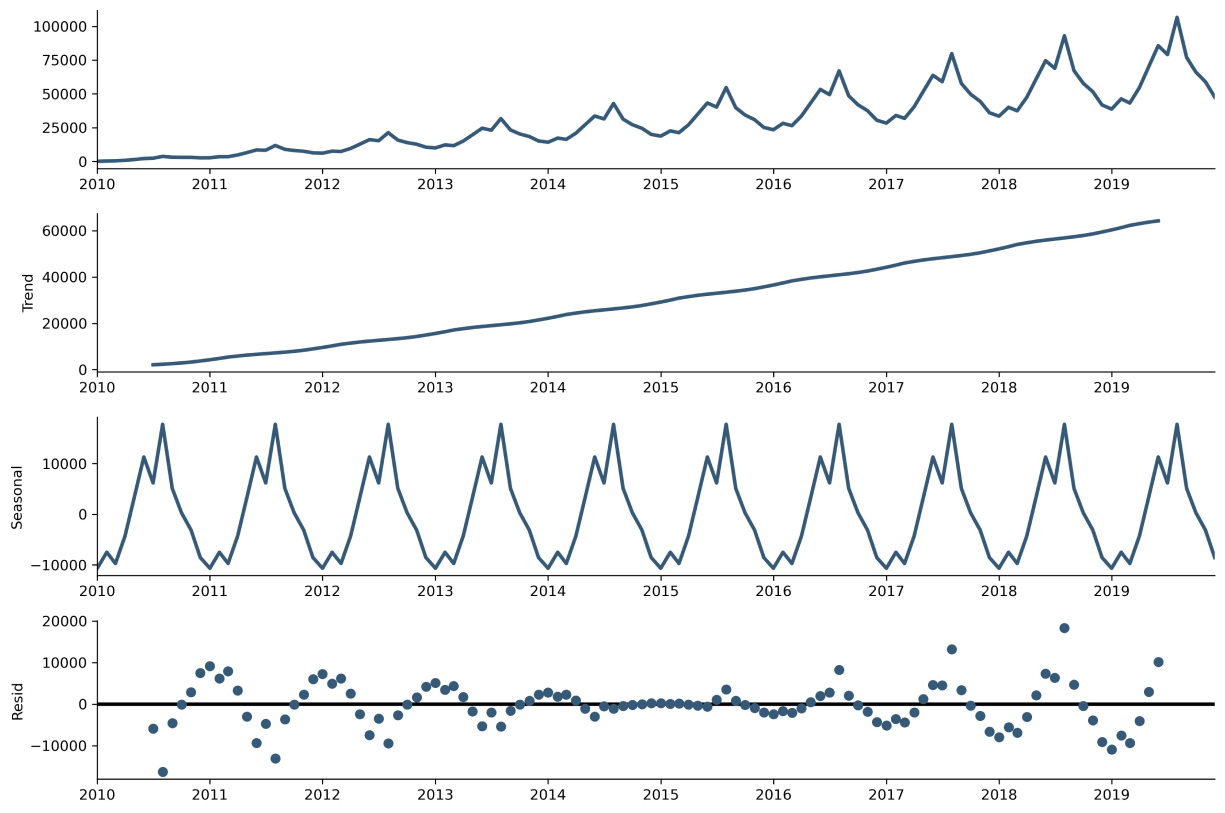
\includegraphics[width=\textwidth]{./figs/illustrations/time-series_example-decomposed.png}
  \hfill
\end{figure}